%!TEX program = xelatex
\documentclass[cn,hazy,blue,14pt,screen]{elegantnote}
\title{Veda:平衡机器算法库工具}

\author{施华}
\institute{Algorithm library tool}

\version{beta-0.1}
\date{\zhtoday}

\usepackage{array}

\begin{document}

\maketitle

\centerline{
  
\includegraphics[width=0.2\textwidth]{logo-ae.png}
}



\section{Veda介绍}

Veda作为算法库管理工具,主要提供了本地库和远端库两套算法库,并提供了本机算法运行环境动态管理以及分布式环境运维的功能。

Veda有下面几个特性:

\begin{itemize}
  \item 本地库与远端库两种管理方式
  \item 算法运行环境动态管理
  \item 算法运行分布式环境运维
\end{itemize}

以下主要是主体框架和基础套餐的设计说明



\subsection{主体框架}

Veda作为算法库管理工具,主要提供了本地库和远端库两套算法库,并提供了本机算法运行环境动态管理以及分布式环境运维的功能主要涉及的技术有:

\begin{enumerate}[label=\arabic*).]
	\item \textit{命令模式}\\
	主体框架采用命令模式
	\item \textit{存储}\\
	本地信息存储使用Sqlite3,包存储使用文件系统;远端信息存储使用ClickHouse,包存储使用Minio.
	\item \textit{管理}\\
	本地环境配置使用Environment Modules;分布式执行使用Ansible.
\end{enumerate}

\centerline{
	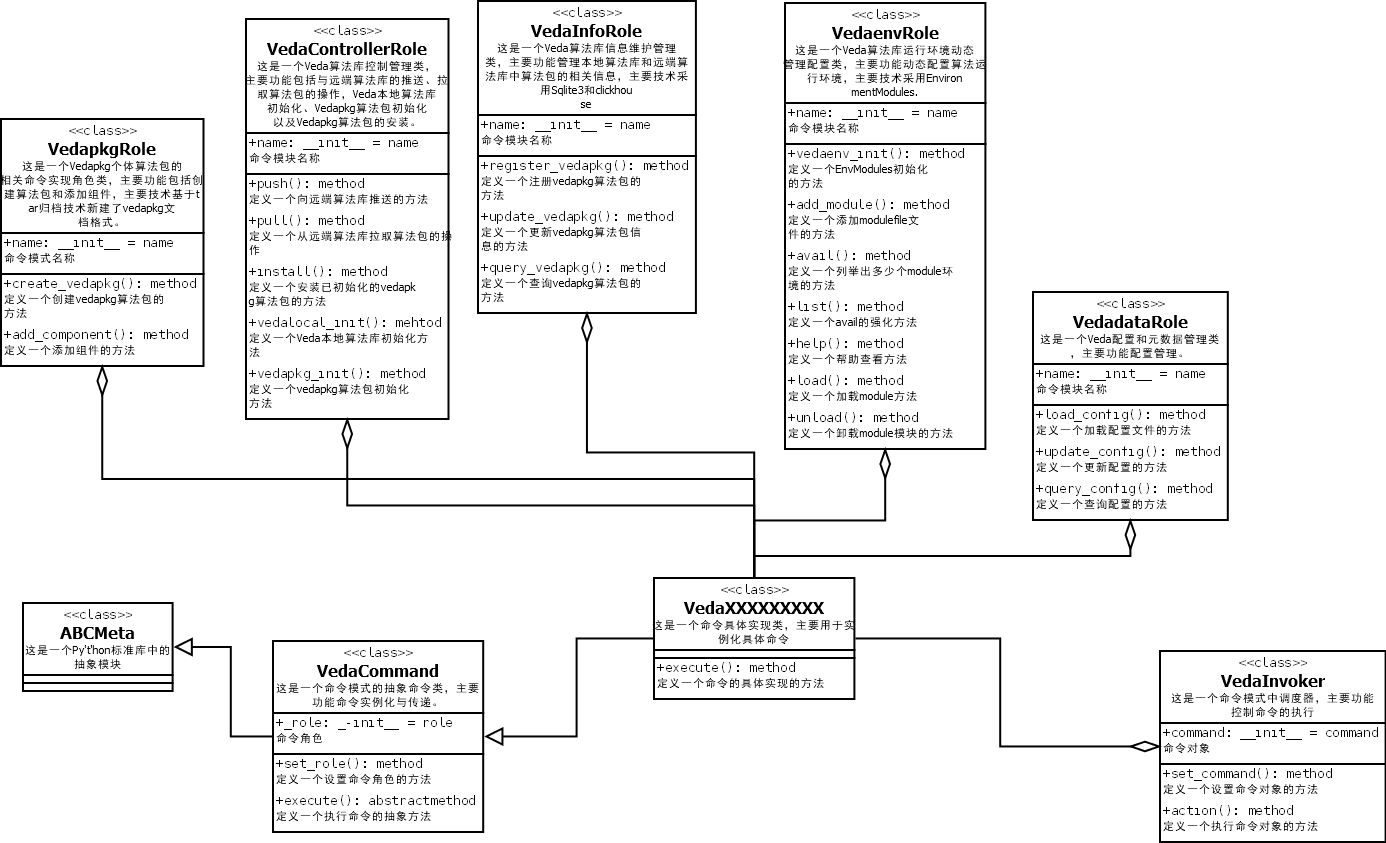
\includegraphics[width=0.8\textwidth]{Veda.png}
}








\subsection{使用示例}

Veda利用click封装了命令行

代码示例:

\begin{lstlisting}
	# 1.veda初始化
	vedainit vedadata --veda_workspace '/home/shihua/tulip/AEwork/Veda/TEST'
	# 2.vedapkg创建工作空间
	vedactl vedapkgcreateworkspace --vedapkg_name 'test_vedapkg_1'
	# 3.vedapkg添加组件
	vedactl vedapkgaddcomponent --vedapkg_name 'test_vedapkg_1' --vedapkg_component_type 'Data' 
	# --vedapkg_component_path '/home/shihua/tulip/AEwork/Veda/Demo/test_veda.py'
	# 4.vedapkg打包
	vedactl vedapkgpack --vedapkg_name 'test_vedapkg_1'
	# 5.vedapkg信息初始化
	vedactl vedapkginfoinit
	# 6.vedapkg本地信息注册
	vedactl vedapkginforegister --name 'test_vedapkg_2' --version 'beta-0.1' --author 'shihua' --summary 'This is a test package' --state 'Test' --requires 'TestPKG'
	# 7.vedapkg本地信息更新
	vedactl vedapkginfoupdate --name 'test_vedapkg_2' --info_key 'version' --info_value 'beta-0.2'
	# 8.vedapkg本地信息查询
	vedactl vedapkginfoquery --name 'test_vedapkg_1'
	# 9.vedainfo远端信息注册
	vedactl vedainforegisterremote --name 'test_vedapkg_2' --version 'beta-0.1' --author 'shihua' --summary 'This is a test package!' --state 'Test' --requires 'TestPKG' --host '10.2.12.248' --port '9000' --clickhouse_user 'admin' --clickhouse_password 'admin'
	# 10.vedainfo远端信息查询
	vedactl vedainfoqueryremote --name 'test_vedapkg_2' --host '10.2.12.248' --port '9000' --clickhouse_user 'admin' --clickhouse_password 'admin'
	# 11.vedainfo远端信息更新
	vedactl vedainfoupdateremote --name 'test_vedapkg_2' --host '10.2.12.248' --port '9000' --clickhouse_user 'admin' --clickhouse_password 'admin' --info_key 'author' --info_value 'shihua_test'
	# 12.vedacontroller远端拉取
	vedactl vedacontrollerpullremote --connect_info '10.2.12.248:9111' --access_key 'minioadmin' --secret_key 'minioadmin' --secure False --object_file 'test_local.vedapkg' --bucket 'vedapkg_remote'
	# 13.vedacontroller远端推送
	vedactl vedacontrollerpushremote --connect_info '10.2.12.248:9111' --access_key 'minioadmin' --secret_key 'minioadmin' --secure False --object_file 'test_local.vedapkg' --bucket 'vedapkg_remote'
	# 14.vedaenv可用环境模板查询
	vedactl vedaenvavail --avail_para 'test'
	# 15.vedaenv已加载环境查询
	vedactl vedaenvlist
	# 16.vedaenv环境模板上传
	vedactl vedaenvload --load_path '/home/shihua/tulip/test/veda/5.2.1' --password 'ATTACK7121553rb1' --target_path '/usr/share/modules/modulefiles/test/5.2.1'
	# 17.vedaenv分布式运维接口
	vedactl vedaenvansible --group 'shihua002' --mode 'shell' --exec_script 'pwd'
\end{lstlisting}



\end{document}
